% \chapter{Contribuția propriu-zisă a candidatului}
\chapter{Arhitectura aplicației}
    \paragraph{} Funcțiile de bază ale acestei aplicații sunt gestionarea containerelor și a imaginilor folosite pentru crearea acestora, și execuția proceselor în aceste medii izolate.
    \paragraph{} Toate fișierele aplicației sunt stocate în directorul \textit{minato} aflat în directorul \textit{/var/lib/} al utilizatorului care rulează aplcația. Acest director conține containerele (\textit{minato/containers}), imaginile (\textit{minato/images}) si alte fișiere auxiliare.
    \begin{figure}[h!]
        \centering
        \begin{forest}
            for tree={
                font=\ttfamily,
                grow'=0,
                child anchor=west,
                parent anchor=south,
                anchor=west,
                calign=first,
                inner xsep=7pt,
                edge path={
                    \noexpand\path [draw, \forestoption{edge}]
                    (!u.south west) +(7.5pt,0) |- (.child anchor) pic {folder} \forestoption{edge label};
                },
                % style for your file node
                file/.style={
                    edge path={
                        \noexpand\path [draw, \forestoption{edge}]
                        (!u.south west) +(7.5pt,0) |- (.child anchor) \forestoption{edge label};
                    },
                    inner xsep=2pt,
                    font=\small\ttfamily
                },
                before typesetting nodes={
                    if n=1
                    {insert before={[,phantom]}}
                    {}
                },
                fit=band,
                before computing xy={l=15pt},
            }
            [ /var/lib
                [ .minato
                    [ containers ]
                    [ images ]
                    [ ..., file ]
                ]
            ]
        \end{forest}
        \caption{Directorul principal al aplicației}
        \label{fig:dirprinc}
    \end{figure}
    \paragraph{} Aplicația este compusă din trei componente principale: Managerul de containere, Managerul de imagini, Daemon/client.

    \pagebreak
    \section{Managerul de containere}
        \paragraph{} Scopul managerului de containere este de a crea o interfață între utilizator și aplicație. Acesta poate efectua următoarele operații:
        \begin{table}[h!]
            \centering
            \begin{tabular}{ |c|l| }
                \hline
                \textbf{Operație} & \textbf{Descrierea operației}  \\
                \hline
                \textit{create} & Crearea unui container  \\
                \hline
                \textit{run}    & Rularea unui container  \\
                \hline
                \textit{open}   & Deschiderea unui container  \\
                \hline
                \textit{stop}   & Oprirea unui container  \\
                \hline
                \textit{list}   & Afișarea tuturor containerelor create  \\
                \hline
                \textit{delete} & Ștergerea unui container  \\
                \hline
            \end{tabular}
            \caption{Operațiile efectuate de către managerul de containere}
            \label{table:cmop}
        \end{table}

        \subsection{Crearea unui container (\textit{create})}
            \paragraph{} Această operație constă în crearea directorului în care se vor stoca fișierele containerului și se va monta sistemul de fișiere. Inițial acesta va conține directoarele necesare pentru operația de montare, \textit{upper}, \textit{lower}, \textit{work} și \textit{merged}, care vor fi goale, cu exceptia directorului \textit{lower}, care va fi o legătură simbolică către directorul în care sunt stocate straturile imaginii care urmează să fiee utilizate de către container.
            \paragraph{} De asemenea, în directorul containerului va fi creat fișierul \textit{config.json} în care se află toate configurările care trebuie aplicate asupra containerului. Printre acestea se regăsesc: maparea unu la unu dintre userul din sistemul de operare și userul din container, \textit{namespaceurile} în care trebuie izolat containerul, hostname-ul containerului, etc.
                \begin{lstlisting}[language=Rust, style=boxed, caption={Crearea unui container},captionpos=b]
pub fn create(&self) -> Result<(), Box<dyn std::error::Error>> {
    info!("creating container");

    if Path::new(&self.path).exists() {
        info!("container exists. skipping creation...");
        return Ok(())
    }
    self.create_directory_structure()?;
    self.generate_config_json()?;

    info!("created container.");
    Ok(())
}               \end{lstlisting}
                \label{fig:cod_ccreate}
            \begin{figure}[h!]
                \begin{subfigure}{.5\textwidth}
                    \centering
                    \begin{forest}
                        for tree={
                            font=\ttfamily,
                            grow'=0,
                            child anchor=west,
                            parent anchor=south,
                            anchor=west,
                            calign=first,
                            inner xsep=7pt,
                            edge path={
                                \noexpand\path [draw, \forestoption{edge}]
                                (!u.south west) +(7.5pt,0) |- (.child anchor) pic {folder} \forestoption{edge label};
                            },
                            % style for your file node
                            file/.style={
                                edge path={
                                    \noexpand\path [draw, \forestoption{edge}]
                                    (!u.south west) +(7.5pt,0) |- (.child anchor) \forestoption{edge label};
                                },
                                inner xsep=2pt,
                                font=\small\ttfamily
                            },
                            before typesetting nodes={
                                if n=1
                                {insert before={[,phantom]}}
                                {}
                            },
                            fit=band,
                            before computing xy={l=15pt},
                        }
                        [ /var/lib
                            [ .minato
                                [ containers
                                    [ cont
                                        [ lower -> /root/.minato/images/...
                                            [ 6154df8ff9882934dc5... ]
                                            [ a3ed95caeb02ffe68cd... ]
                                            [ ..., file ]
                                        ]
                                        [ merged ]
                                        [ upper ]
                                        [ work ]
                                        [ config.json, file]
                                    ]
                                ]
                                [ ..., file ]
                            ]
                        ]
                    \end{forest}
                    \caption{Directorul unui container}
                    \label{fig:dircont}
                \end{subfigure}
                \begin{subfigure}{.5\textwidth}
                    \centering
                    \begin{forest}
                        for tree={
                            font=\ttfamily,
                            grow'=0,
                            child anchor=west,
                            parent anchor=south,
                            anchor=west,
                            calign=first,
                            inner xsep=7pt,
                            edge path={
                                \noexpand\path [draw, \forestoption{edge}]
                                (!u.south west) +(7.5pt,0) |- (.child anchor) pic {folder} \forestoption{edge label};
                            },
                            % style for your file node
                            file/.style={
                                edge path={
                                    \noexpand\path [draw, \forestoption{edge}]
                                    (!u.south west) +(7.5pt,0) |- (.child anchor) \forestoption{edge label};
                                },
                                inner xsep=2pt,
                                font=\small\ttfamily
                            },
                            before typesetting nodes={
                                if n=1
                                {insert before={[,phantom]}}
                                {}
                            },
                            fit=band,
                            before computing xy={l=15pt},
                        }
                        [ /var/lib
                            [ .minato
                                [ containers
                                    [ cont
                                        [ merged
                                            [ bin ]
                                            [ boot ]
                                            [ dev ]
                                            [ etc ]
                                            [ home ]
                                            [ ..., file ]
                                        ]
                                        [ ..., file ]
                                        [ pid, file ]
                                    ]
                                ]
                                [ ..., file ]
                            ]
                        ]
                    \end{forest}
                    \caption{Directorul unui container în timpul rulării}
                    \label{fig:controot}
                \end{subfigure}
                \caption{Directorul unui container}
                \label{fig:dircontfig}
            \end{figure}

        \subsection{Rularea unui container (\textit{run})} \label{section:run}
            \paragraph{} Operația de rulare reprezintă crearea propriu-zisă a spațiului izolat în sistemul de operare. Pentru realizarea acestei operații, se efectuează mai mulți pași.
            \begin{lstlisting}[language=Rust, style=boxed, caption={Rularea unui container},captionpos=b]
fn run(&self, daemon: bool, volume: Option<String>) -> Result<(), Box<dyn std::error::Error>> {
    self.mount_container_filesystem()?;
    self.prepare_container_mountpoint()?;
    self.mount_volume(volume)?;
    self.prepare_container_directories()?;
    self.prepare_container_networking()?;
    self.mount_container_directories()?;
    self.prepare_container_id_maps()?;
    self.pivot_container_root()?;
    self.execute_inner_fork(daemon)?;

    Ok(())
}           \end{lstlisting}
            \label{fig:cod_crun}
            \begin{figure}[h!]
                \centering
                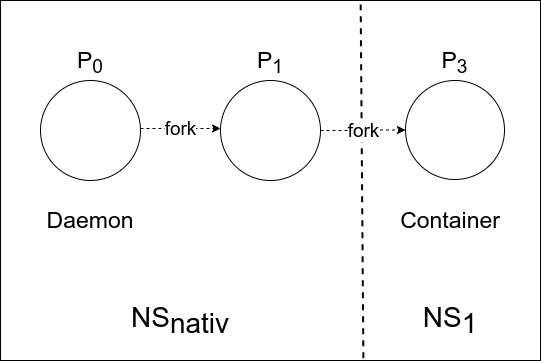
\includegraphics[width=.75\textwidth]{fork}
                \caption{Crearea procesului în noul namespace}
                \label{fig:fork}
            \end{figure}
            \paragraph{Efectuarea primului \textit{fork},} care are rolul de a separa procesul containerului de procesul \textit{daemonului} atunci cănd programul trebuie sa ruleze pe fundal și de a îl păstra pe acesta în \textit{namespaceul} inițial al sistemului de operare gazdă. De asemenea, este creat fișierul \textit{pid} care este folosit pentru a verifica daca container-ul rulează deja și, în cazul afirmativ, care este PID-ul acestuia. Crearea fișierului este efectuată de către părintele din \textit{fork}, resul pașilor de către copil.
            \paragraph{Montarea rădăcinii containerului,} cu sistemul de fișiere OverlayFS folosind comanda \textbf{mount -t overlay overlay -olowerdir=/lower,upperdir=/upper,\\workdir=/work /merged}. În urma acesteia, în directorul \textit{merged} se va găsi structura de directoare specifică \textit{kernelului} Linux.
            \begin{lstlisting}[language=Rust, style=boxed, caption={Montarea directorului în care este sistemul de fișiere al containerului},captionpos=b]
fn mount_container_filesystem(&self) -> Result<(), Box<dyn std::error::Error>> {
    info!("mounting container filesystem...");

    let container_path = Path::new(&self.path);
    let subdirectories = container_path.join("lower")
        .read_dir().unwrap()
        .map(|dir|
            format!("{}", dir.unwrap().path().display()))
        .collect::<Vec<String>>()
        .join(":");
    let lowerdir_arg  = format!("lowerdir={}",       subdirectories);
    let upperdir_arg  = format!("upperdir={}/upper", &self.path);
    let workdir_arg   = format!("workdir={}/work",   &self.path);
    let mergeddir_arg = format!("{}/merged",         &self.path);
    let full_arg = format!("{},{},{}",
        lowerdir_arg, upperdir_arg, workdir_arg
    );

    mount(
        Some("overlay"),
        mergeddir_arg.as_str(),
        Some("overlay"),
        MsFlags::empty(),
        Some(full_arg.as_str())
    )?;

    info!("mounted container filesystem.");
    Ok(())
}           \end{lstlisting}
            \label{fig:cod_cmount}
            \paragraph{Apelul funcției \textit{unshare}} cu \textit{flag}-urile specifice fiecarui \textit{namespace}. În urma acestuia, toate procesele copil ale procesului curent vor fi create în \textit{namespace}-uri separate.
            \paragraph{Setarea sistemului de fișiere al mașinii gazdă ca privat.} Acest pas are rolul de a izola toate evenimentele de montare sau de demontare care au loc în sistemul de operare gazdă.
            \paragraph{Legarea executabilului folosit ca proces inițial (init).} Acest pas constă în efectuarea unui \textit{bind mount} între fișierul \textit{tini}, aflat în directorul \textit{.minato}, și un fișier nou creat în sistemul de fișiere al containerului. \textit{tini} este un program open-source care are aceleași funcționalitați ca procesul \textit{init} găsit în sistemele de operare Unix, de exemplu, protecția împotriva creării proceselor \textit{zombie}.
            \paragraph{Crearea directoarelor} \textit{dev}, \textit{sys}, \textit{proc}, \textit{old\_proc} și \textit{put\_old}. Directoarele \textit{dev}, \textit{sys} și \textit{proc} conțin sisteme de fișiere specifice sistemelor de operare Unix, necesare pentru funcționarea containerului. Directorul \textit{old\_proc} este folosit pentru montarea pseudo-sistemului de fișiere \textit{proc}, iar directorul \textit{put\_old} este folosit în operația de schimbare a rădăcinii procesului curent, \textit{pivot\_root}.
            \paragraph{Crearea legăturii de rețea} dintre container și sistemul de operare gazdă folosind un dispozitive virtuale de \textit{ethernet}(\textit{veth}) și un \textit{bridge}. În executarea acestei operații se foloseste aplicația \textbf{iproute2} din kernelul Linux.
            \begin{lstlisting}[language=bash, style=boxed, caption={Comenzile utilizate pentru crearea legăturii de rețea},captionpos=b]
ip link add example-br0 type bridge
ip link set dev example-br0 up
ip link add example-veth0 type veth peer name example-veth1
ip addr add 192.168.1.10/24 dev example-veth0
ip link set example-veth0 up
ip link set dev example-veth1 master example-br0
ln /proc/67539/ns/net /var/run/netns/example-ns
ip link set example-veth1 netns example-ns
ip netns exec example-ns ip link set lo up
ip netns exec example-ns ip link set example-veth1 up
ip netns exec example-ns ip addr add 192.168.1.11/24 dev example-veth1
ip netns exec example-ns ip route add default via 192.168.1.11/24 \end{lstlisting}
                \label{fig:cod_net}
            \paragraph{Montarea directoarelor \textit{dev} și \textit{proc}, și a ierarhiei cgroup.} Directorul \textit{dev} va fi legat cu cel din sistemul gazdă pentru a avea acces la dispozitivele acesteia, iar directorul \textit{proc} va fi de asemenea legat cu cel din sistemul gazdă, dar doar temporar. Pentru crearea ierarhiei cgroup este nevoie doar de crearea și montarea directoarelor principale ( \textit{freezer}, \textit{memory}, \textit{blkio}, etc.) ale acesteia. Odata montate, acestea sunt populate automat de către \textit{kernel}.
            \begin{lstlisting}[language=Rust, style=boxed, caption={Montarea directoarelor \textit{dev} și \textit{proc}, și a ierarhiei cgroup},captionpos=b]
fn mount_container_directories(&self) -> Result<(), Box<dyn std::error::Error>> {
    info!("mounting container directories...");

    info!("mounting proc to old_proc...");
    mount(
        Some("/proc"),
        "old_proc",
        None::<&str>,
        MsFlags::MS_BIND | MsFlags::MS_REC,
        None::<&str>,
    )?;

    self.mount_container_cgroup_hierarchy()?;

    info!("mounting dev to dev...");
    mount(
        Some("/dev"),
        "dev",
        None::<&str>,
        MsFlags::MS_BIND | MsFlags::MS_REC,
        None::<&str>,
    )?;

    info!("mounted container directories.");
    Ok(())
}

fn mount_container_cgroup_hierarchy(&self) -> Result<(), Box<dyn std::error::Error>> {
    info!("mounting container cgroup hierarchy...");

    let directories = vec![
        "freezer", "hugetlb", "memory", "blkio", "cpuset",
        "cpu,cpuacct", "devices", "pids",
        "net_cls,net_prio", "perf_event", "rdma"
    ];

    for dir in directories {
        let dir_path = format!("sys/fs/cgroup/{}", dir);
        if Path::new(&dir_path).exists() {
            fs::remove_dir_all(&dir_path)?;
        }
        fs::create_dir_all(&dir_path)?;

        info!("mounting cgroup {}...", dir);
        let cgroup_version = "cgroup";
        mount(
            Some(cgroup_version),
            dir_path.as_str(),
            Some(cgroup_version),
            MsFlags::MS_NOSUID | MsFlags::MS_NODEV | MsFlags::MS_NOEXEC,
            Some(dir),
        )?;
    }

    info!("mounted container cgroup hierarchy.");
    Ok(())
}           \end{lstlisting}
            \label{fig:cod_mount2}
            \paragraph{Schimbarea id-urilor utilizatorului} pentru noul \textit{user namespace}, folosind fișierele \textit{/proc/self/uid\_map} și \textit{/proc/self/gid\_map}. Acestea permit crearea unei legături unu la unu între id-urile din sistemul de operare gazdă si id-urile din container. După crearea unui \textit{user namespace} nou, fișierul \textit{uid\_map} al containerului poate fi scris o singură dată pentru a defini maparea ID-urilor utilizatorului în noul spațiu de utilizator. Încercarea de a scrie de mai multe ori într-un fișier \textit{uid\_map} dintr-un \textit{user namespace} eșuează cu eroarea EPERM. Reguli similare se aplică pentru fișierul \textit{gid\_map}. \cite{ns:user}
            \paragraph{Schimbarea rădăcinii sistemului de fișiere} din container folosind operația \textit{pivot\_root}. Directorul \textit{put\_old} este un director aflat în rădacina containerului, necesar pentru această operația. Odata folosit, el este demontat si șters.
            \begin{lstlisting}[language=Rust, style=boxed, caption={Schimbarea rădăcinii sistemului de fișiere},captionpos=b]
fn pivot_container_root(&self) -> Result<(), Box<dyn std::error::Error>> {
    info!("pivoting container root..");

    info!("pivoting root...");
    pivot_root(".", "put_old")?;

    info!("unmounting pivot auxiliary folder...");
    umount2("/put_old", MntFlags::MNT_DETACH)?;
    if Path::new("/put_old").exists() {
        info!("removing auxiliary folder...");
        std::fs::remove_dir_all("/put_old")?;
    }

    info!("pivoted container root.");
    Ok(())
    }           \end{lstlisting}
                \label{fig:cod_mount2}

            \paragraph{Efectuarea \textit{fork}-ului final} pentru aplicarea efectelor operației \textit{unshare}. Acesta va crea un nou proces copil, în care se va executa primul proces al containerului folosind comanda \textit{execve}.
            \paragraph{Curățarea spațiului de lucru} urmată de sfârșirea procesului început de către container. Aceasta constă în ștergerea dispozitivelor create pentru stabilirea legăturii de rețea dintre container și sistem de operare, și în demontarea sistemului de fișiere \textit{overlay}.

            \begin{figure}[h!]
                \centering
                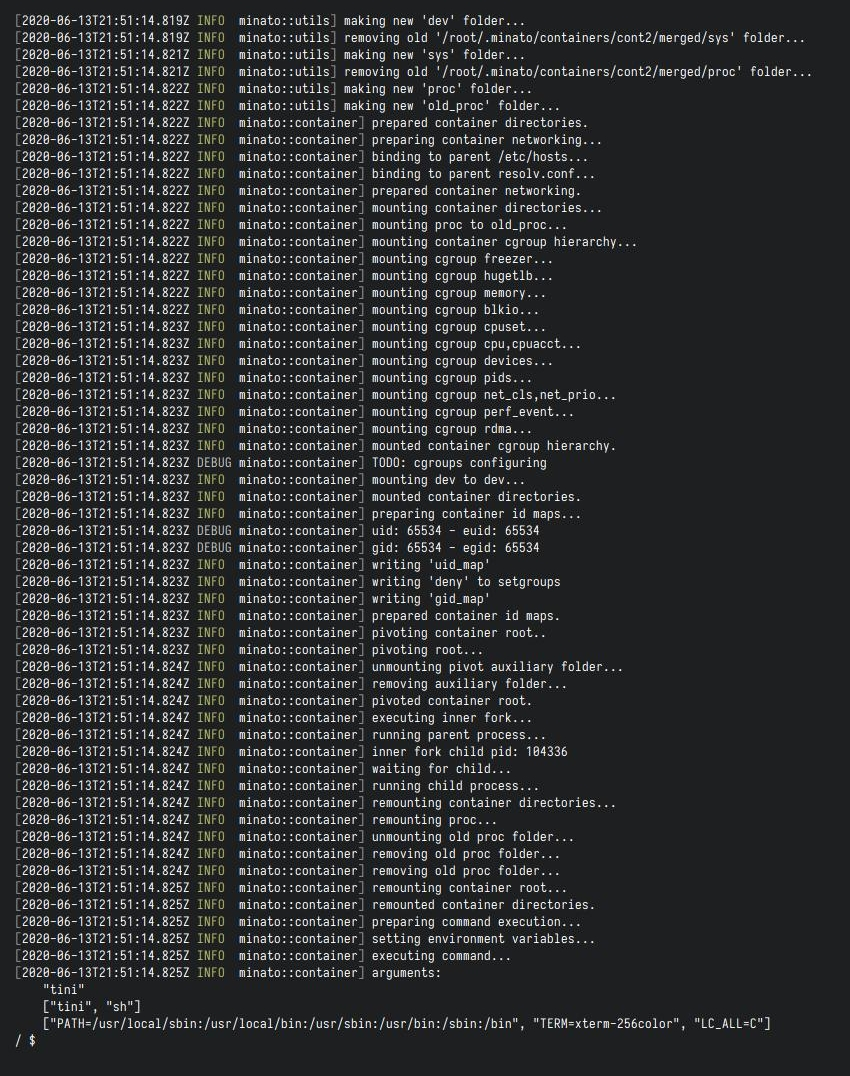
\includegraphics[width=1\textwidth]{cont_run}
                \caption{Rularea unui container cu comanda /bin/sh}
                \label{fig:run}
            \end{figure}

        \pagebreak
        \subsection{Deschiderea unui container (\textit{open})}
            \paragraph{} Operația de deschidere a unui container se realizează folosind apelul de system \textit{setns} împreuna cu \textit{flag}-urile specifice fiecarui \textit{namespace}, urmat de comanda \textit{execve} cu interpretorul \textit{sh}.
                \begin{lstlisting}[language=Rust, style=boxed, caption={Deschiderea unui container},captionpos=b]
pub fn open(&self, container_name: &str) -> Result<(), Box<dyn std::error::Error>> {
    info!("opening container...");

    let container_pid = match utils::get_container_pid_with_str(container_name).unwrap() {
        None => {
            info!("container isn't running or doesn't exist. exiting...");
            return Ok(());
        },
        Some(pid) => pid
    };
    info!("container pid: {}", container_pid);
    let mut namespaces = HashMap::new();
    namespaces.insert(CloneFlags::CLONE_NEWIPC, "ipc");
    namespaces.insert(CloneFlags::CLONE_NEWUTS, "uts");
    namespaces.insert(CloneFlags::CLONE_NEWNET, "net");
    namespaces.insert(CloneFlags::CLONE_NEWPID, "pid");
    namespaces.insert(CloneFlags::CLONE_NEWNS, "mnt");
    namespaces.insert(CloneFlags::CLONE_NEWCGROUP, "cgroup");
    namespaces.insert(CloneFlags::CLONE_NEWUSER, "user");
    let pid_path = format!("/proc/{}/ns", container_pid);
    info!("setting namespaces...");
    for namespace in namespaces {
        let ns_path = format!("{}/{}", pid_path, namespace.1);
        self.set_namespace(ns_path.as_str(), namespace.0)?;
    }
    let result = match fork() {
        Ok(ForkResult::Parent { child, .. }) => {
            waitpid(child, None)?;
            Ok(())
        }
        Ok(ForkResult::Child) => {
            self.do_exec("/bin/sh")
        }
        Err(e) => {
            info!("fork failed: {}", e);
            Ok(())
        }
    };
    info!("opened container.");
    result
}                \end{lstlisting}
                \label{fig:cod_ccreate}

        \subsection{Oprirea unui container (\textit{stop})}
            \paragraph{} Operația de oprire a unui container se realizează folosind apelul de system \textit{kill} împreuna cu \textit{flag}-ul \textit{SIGTERM} și id-ul PID al container-ului.

        \subsection{Afișarea tuturor containerelor create (\textit{list})}
            \paragraph{} Operația de afișare a containerelor se realizează prin citirea tuturor directoarelor aflate în directoarele \textit{containers} și \textit{images}. Pentru fiecare container găsit se afișeaza numele acestuia, imaginea folosită pentru crearea lui, locația unde este stocat și PID-ul lui dacă acesta rulează.

        \subsection{Ștergerea unui container (\textit{delete})}
        \paragraph{} Operația de ștergere a unui container se realizează prin ștergerea directorului în care acesta este stocat.

    \section{Managerul de imagini}
        \paragraph{} Asemănător cu managerul de containere, scopul managerului de imagini este de a crea o interfață între utilizator și aplicație. Acesta poate efectua următoarele operații:
        \begin{table}[h!]
            \centering
            \begin{tabular}{ |c|l| }
                \hline
                \textbf{Operație} & \textbf{Descrierea operației}  \\
                \hline
                \textit{pull}   & Downloadarea și stocarea unei imagini  \\
                \hline
                \textit{list}   & Afișarea tuturor imaginilor downloadate  \\
                \hline
                \textit{delete} & Ștergerea unei imagini  \\
                \hline
            \end{tabular}
            \caption{Operațiile efectuate de către managerul de containere}
            \label{table:cmop}
        \end{table}

        \subsection{Downloadarea și stocarea unei imagini (\textit{pull})}
            \paragraph{} Downloadarea imaginilor se face din \textit{repository}-ul Docker, Docker Hub, prin API-ul pus la dispoziție de către aceștia. Acest proces constă în autentificarea cu API-ul și downloadarea fișierului \textit{json} asociat imaginii. Din acest fișier sunt extrase date pentru descărcarea straturilor imaginii, care apoi sunt descărcate și dezarhivate în directorul imaginii.

        \subsection{Afișarea tuturor imaginilor downloadate (\textit{list})}
            \paragraph{} Operația de afișare a imaginilor se realizează prin citirea tuturor directoarelor aflate în directorul \textit{images}. Pentru fiecare imagine găsită se afișeaza numele acesteia locația unde este stocată.

        \subsection{Ștergerea unei imagini (\textit{delete})}
        \paragraph{} Operația de ștergere a unei imagini se realizează prin ștergerea directorului în care aceasta este stocată.

    \section{Daemon/client}
        \paragraph{} Componenta daemon/client permite rularea unui proces pe fundal care se ocupă cu gestionarea containerelor și a imaginilor, și comunicarea cu acesta.
        \paragraph{} Beneficiul principal al acestei componente este faptul că aceasta pune la dispoziție accesul la operațiile containerului și utilizatorilor neprivilegiați.
        \paragraph{} Comunicarea dintre client și daemon are loc prin \textit{socketuri} Unix, daemonul așteptănd constant să primească instrucțiuni de la clienți pe care apoi să le execute. Clienții pot trimite operații specifice programului, printre care și cea de oprire a daemon-ului.


% \section{Arhitectura aplicatiei}
%     \subsection{pachete de clase pentru partea de user/admin}
%     \subsection{diagrama entitate relatie a bazei de date}
%     \subsection{alte componente incapsulate (maps, API-uri etc)}
% \section{Structurată în funcție de tipul lucrării, fiind compusă dintr-un număr arbitrar de capitole (vezi formatul lucrării în funcţie de tip).}
%     \subsection{Descriu în detaliu fundamentarea teoretică și dezvoltarea aplicativă (dacă e cazul) a temei abordate}
%     \subsection{Conţin puncte de vedere personale, interpretări ale teoriilor și conceptelor abordate în lucrare}
%     \subsection{Trec în revistă abordări existente ale problemei cu evidențierea avantajelor şi dezavantajelor}
%     \subsection{Descompun problema propusă de tema lucrării în subprobleme specifice şi prezentarea modului de rezolvare, analize critice ale fenomenelor şi proceselor studiate, comparații cu rezultate obţinute anterior (unde e cazul), proiectarea aplicaţiei, detalii de implementare, rezultate experimentale, exemple de test sau rezultate sub forma unor studii de caz, modul de utilizare a programului etc.}
% \section{Functionalitatea aplicatiei}
%     \subsection{un ghid al aplicatiei cu capturi de imagine si secvente de cod reprezentative}
% \section{Testarea aplicatiei}
%     \subsection{teste functionale}
%     \subsection{identificarea unor puncte slabe care vor fi rezolvate ulterior}